\documentclass[conference]{IEEEtran}
\usepackage{cite}
\usepackage{amsmath,amssymb,amsfonts}
\usepackage{algorithmic}
\usepackage{graphicx}
\usepackage{textcomp}
\usepackage{xcolor}
\def\BibTeX{{\rm B\kern-.05em{\sc i\kern-.025em b}\kern-.08em
		T\kern-.1667em\lower.7ex\hbox{E}\kern-.125emX}}


\usepackage{diagbox}
\usepackage{amsthm}
\usepackage[formats]{listings}
\graphicspath{{images/}}
\DeclareGraphicsExtensions{.pdf,.png,.jpg}
\theoremstyle{plane}
\newtheorem{theorem}{Theorem}[section]

\begin{document}

\title{Unified data structures to optimize solving a complex of interrelated geometric problems*\\
%{\footnotesize \textsuperscript{*}Note: Sub-titles are not captured in Xplore and should not be used}
%\thanks{Identify applicable funding agency here. If none, delete this.}
}
\author{
\IEEEauthorblockN{1\textsuperscript{st} Vasyl Tereshchenko}
\IEEEauthorblockA{\textit{Faculty of computer science and cybernetics} \\
\textit{Taras Shevchenko National University of Kyiv}\\
Kyiv , Ukraine \\
vtereshch@gmail.com}
\and
\IEEEauthorblockN{2\textsuperscript{nd} Semen Chudakov}
\IEEEauthorblockA{\textit{Faculty of computer science and cybernetics} \\
\textit{Taras Shevchenko National University of Kyiv}\\
Kyiv , Ukraine \\
semen.chudakov7@gmail.com}
}
\maketitle

\begin{abstract}
The paper is devoted to the development of an efficient algorithmic tools for solving a set of interrelated computational geometry problems. To do this, a single algorithmic environment with unified data structures is created, which allows to implement complex use cases efficiently with respect to computational resources. We build the environment on the basis of the ``divide and conquer'' strategy. 
Once a convex hull is key to a set of computational geometry problems, we offer a special weighted concatenable queue data structure to maintain it. The data structure is implemented in a form of a binary tree. This allows to perform operations needed in algorithm for a set of tasks within no more than $O(\log n)$ time. Furthermore we offer a way to execute the algorithms both sequentially and in parallel.
In the future the algorithmic environment can be improved to support other \textcolor{blue}{computational models} with similar properties for solving problems. As an example, the Voronoi Diagram or the Delaunay Triangulation can be considered.
\end{abstract}

\begin{IEEEkeywords}
Algorithmic tools,   Computational geometry, Interrelated problems set, Single algorithmic environment, A weighted concatenable queue
\end{IEEEkeywords}

\section{Introduction}

Nowadays, advanced computer simulations and visualizing of complex scientific researches as well as large scale technical projects requires to simultaneously solve a set of \textcolor{red}{science and technology objectives}. The core of this set are problems of computational geometry and computer graphics. To solve such problems it is needed to create suitable algorithmic frameworks, that would yield accurate results in real time. Existing methods (iLastic[1], IMARIS [2], ImageJ (або FiJi) [3]), that are based on set of algorithms implementations organized in a package does not result in desirable efficiency and accuracy. It is worse noting, that there are a lot of parallel algorithms designed to solve specifically certain computational geometry problems [4-14]. Every such algorithm requires its own computational resources and is executed independently from others. In such case some identical steps, such as precomputation and building data structures, are performed several times. 

Therefore, a important objective in developing of the algorithmic models is to create a universal tool, which would have means to efficiently solve a problems in the set. This tool should also execute identical steps of the algorithms once and be able to represent results of those steps in a form of the common data structures. In [15] the notion of a single algorithmic environment is introduced, which is based on the ``divide-and-conquer'' principle and takes into account the aforementioned features of the algorithms. In particular, the precomputation and splitting the initial set of data to form the recursion tree is common for all the problems is as s result is executed only once. During the merge stage the intermediate results are maintained in the weighted concatenable queue. This model does not repeat computations and the intermediate results are highly reused during the algorithms, which yields good performance.

\textcolor{blue}{This article provides detailed explanation on how the common data structures from [15] are implemented on the example of a convex hull algorithm.}

\section{Convex hull algorithm}
\subsection{Problem statement}

The notion of a convex hull is simple. For a set of points $S$ in a $k$-dimensional space it is a smallest convex set, that comprise $S$. In practice to solve such problem, means to find a subset in $S$, which can be a "skeleton" for the convex hull.

\subsection{Concatenable queue}

Concatenable queue is an Abstract Data Type (ADT), that supports following operations:

\begin{itemize}
	\item
	ADD\_ELEMENT();
	\item
	REMOVE\_ELEMENT();
	\item
	GET\_MINIMUM();
	\item
	CONTAINS();
	\item
	SPLIT();
	\item
	MERGE().
\end{itemize}

By default the elements in a concatenable queue are kept i a certain predefined order \cite{aho}.

Here the concatenable queue is implemented as a binary  $B+$ tree. Its elements are divided into non-leaf and leaf elements. The leaf elements contain all data kept in a tree. Every element has a pointer to its left and right child element. For the leaf elements those pointers point to the elements left and right neighbors or $null$ if the element is utmost in the tree. 
Additionally every element keep a pointer to the largest element in its left sub-tree, which  allows to perform binary search \cite{aho}.  An example of such tree is given on fig. 1. The height of earch element is kept for the balancing process during the split and merge operations. It is measured as a maximum amount of steps it is possible to do in order to reach a leaf element.

\begin{figure}[htbp]
	\centerline{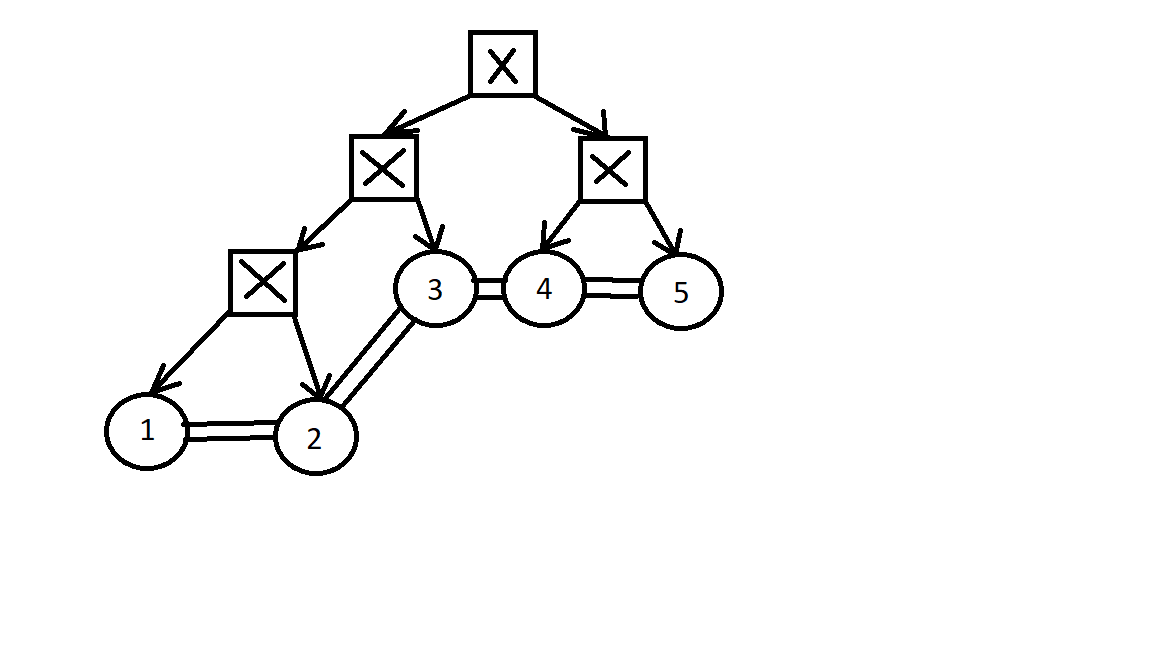
\includegraphics[width=0.4\textwidth, height=0.2\textheight]{cq_example}}
	\caption{Example of a concatenable queue.}
	\label{cq_example}
\end{figure}

From now we will go into details on how this data structure is implemented. So on the list. 1 its formal definition is provided:

\begin{figure}[htbp]
	\begin{lstlisting}[caption={Structure of a concatenable queue vertex},captionpos=b]
	class Node:
	int data		
	int height
	
	Node left
	Node right
	Node leftSubtreeMax
	
	boolean isLeaf
	
	class ConcatenableQueue:
	Node root
	Node minNode
	Node maxNode
	\end{lstlisting}
\end{figure}

The contains operations uses binary search by the tree elements so its complexity is $O(\log n)$, where $n$ hereafter denotes the numbers of elements in the queue.

Algorithm of insertion an element in a queue looks like as follows. First, the position of a new element is searched. Then the connections between adjacent leaf elements are broken to insert a new element. Going back a new non-leaf element is created - parent for the new element and one of its neighbor. The algorithm is formally described on the list. 2.

\begin{figure}[htbp]
\begin{lstlisting}[caption={Queue element insertion algorithm},captionpos=b]
Node insert(Node node, int e):
Node result = nil
if e <= node.leftSubtreeMax.data: 
if node.isLeaf:
if e == node.data:
node.data = e
else:
Node createdLeaf = 
createLeafBetween(e, node.left, node)
result = 
Node(createdLeaf, createdLeaf, node)
else:
node.left = insert(node.left, e)
else:
if node.isLeaf: 
Node createdLeaf = 
createLeafBetween(e, node, node.right)
result = Node(node, node, createdLeaf)
else: 
// go left and update node.right pointer
node.right = insert(node.right, e)

if result == nil:
result = node

updateHeight(result)
return result
\end{lstlisting}
\end{figure}
	
The \textit{updateHeight} subroutine updates the value of an element height, the \textit{createLeafBetween} subroutine breaks the connection between adjacent elements and insertion of a new one. 

The \textit{insert} operation. On the first step we find out if $leftSubtreeMax$ point to an element with greater value than the value to be inserted $e$. If so, then if current element is a leaf, a new element is created between the current element and its left neighbor. Otherwise the search proceeds on the left sub-tree of the current element. The case, when $leftSubtreeMax$ is smaller than the value $e$ is analogous. The procedure ends with updating the height on a newly created element. The element is returned as its result value.

Since on every step we perform a constant amount of work, the complexity of the procedure is $O(h)=O(\log n)$, where $h$ hereafter denotes the height of the tree.

The operation of removing an element from the queue is performed analogously. 

The split operation is a bit more complex. As an input the corresponding procedure receives current element and value based on which the split is performed. As a result two independent queues are formed. The value, by which the split has been performed, belongs to the left sub-queue. The procedure is described formally on the list. 3.

\begin{lstlisting}[caption={Queue plit algorithm},captionpos=b]
split(Node node, int e, 
ConcatenableQueue leftQueue, 
ConcatenableQueue rightQueue): 
if node.isLeaf
leftQueue.root = node
leftQueue.maxNode = node	

rightQueue.minNode = node.right	
cut(node)
else:
if e == node.leftSubtreeMax.data:
leftQueue.root = node.left
leftQueue.maxNode = node.leftSubtreeMax

rightQueue.root = node.right
rightQueue.minNode = node.leftSubtreeMax.right

cut(node.leftSubtreeMax)
else if e < node.leftSubtreeMax.data:
split(node.left, e, leftQueue, rightQueue)
rightQueue.root =
concatenateNodes(rightQueue.root, 
node.right, node.leftSubtreeMax)
else:
split(node.right, e, leftQueue, rightQueue)
leftQueue.root = 
concatenateNodes(node.left, 
leftQueue.root, node.leftSubtreeMax)
\end{lstlisting}

Here the $concatenateNodes$ procedure is used. It performs concatenation of two arbitrary elements and uses theirs heights to balance the resulting queue. Its implementation is described further in the work. The $cut$ procedure breaks connection between two adjacent leaf elements in a queue and therefore is trivial. On the first step in the $split$ operation we check, is the current element is a leaf. Is so, its connection are broken and the value of $maxNode$ is updated for the left queue as well as the value of $minNode$ for the right queue. If element is not a leaf, then the procedure continues of either left or right sub-tree. Here a special corner cases is considered, where $leftSubtreeMax$ contain the dividing value. Then the analogous action to the usual search are performed.


The algorithm of the $concatenateNodes$ procedure is described on the list. 4.

\begin{lstlisting}[caption={Merging two queues using heights},captionpos=b]
Node concatenateNodes(Node leftNode, 
Node rightNode, Node leftSubtreeMax) {
if leftNode == nil:
return rightNode
else if rightNode == nil: 
return leftNode
else if leftNode.height == rightNode.height:
Node result = Node(leftSubtreeMax, 
leftNode, rightNode)
updateHeight(result)
return result
else if leftNode.height < rightNode.height:
rightNode.left = concatenateNodes(leftNode, 
rightNode.left, leftSubtreeMax)
updateHeight(rightNode)
return rightNode
else
leftNode.right = 
concatenateNodes(leftNode.right, 
rightNode, leftSubtreeMax)
updateHeight(leftNode)
return leftNode
\end{lstlisting}

First, we consider corner cases where one of the elements is $null$. This is required to ensure correctness of the recursion. Then, if the left element is higher than the right, one step down is taken for the left element. If the right element is higher - we take a step down for it. If the heights are equal, the joining point is found and a new element must be created. At each step, it is necessary to update the height of current element as it changes.

We begin by analyzing the complexity of the $split$ procedure by determining the complexity of the $concatenateNodes$ procedure. At each iteration, the step is performed either to the left son of the current element or to the right. The execution of the recursive procedure is finished by merging two elements. Since each step moves us down one level and a constant amount of work is performed for each level, the total complexity of the $concatenateNodes$ procedure is $O(h)=O(\log n)$.

The $split$ procedure uses the $concatenateNodes$ function as a subroutine. The complexity a $split$ call is equal to the complexity of $concatenateNodes$. The number of recursive calls $split$ for one split is $\log n$, so the total complexity of the procedure $\log^2 n$.

The merge operation of two queues is reduced to the clamping of their root vertices by the $concatenateNodes$ procedure, so its complexity is $O(\log n)$.

\subsection{Precomputation}

In the pre-processing stage, the "inner" points, which lie on a horizontal or vertical line, are removed from the set. Formally, the removal criterion is formulated as follows. For $a = (x_a, y_a)$ we denote $x(a)=x_a$, $y(a)=y_a$. Let points $a_1, a_2, ..., a_k$ lie on one horizontal line and $x(a_1) < x(a_2) <... <x (a_k) $. Then, by the criterion, the points $a_2, a_3, ..., a_{k-1}$ must be removed. Similarly for the vertical case.

Consider an algorithm that, in a sorted array, for each group of identical elements, deletes all but the first and the last (if the repetition is more than two). The description of the algorithm is given in Listing 5.

\begin{lstlisting}[caption={Algorithm of removing duplicates in a sorted array},captionpos=b]
removeDuplicated(int[] points) {
int n = points.length

if n == 0:
return

it1 = 1
it2 = 0

while it2 < n:
if it2 + 1 > 0 && it2 + 1 < n - 1:
int previous = points[it2-1]
int current = points[it2]
int next = points[it2+1]

if previous != current || current != next:
points[it1] = current
if it1 < n-1:
++it1
else if it2 + 1 == 0:
if it1 < n-1:
++it1
++it2
else:
points[it1] = points[it2]

if it1 < n-1:
while it1 + 1 != points.length:
delete points[n - 1]
\end{lstlisting}

The idea behind the algorithm is to use two pointers to delete repetitions by overwriting their place with other non-repeating element. In this way, additional memory usage can be reduced to a constant value. The algorithm makes one pass through the array. At each step, a constant amount of work is performed to decide whether to delete the current item. Given this, the complexity of the above algorithm is $O(n)$.

To perform the above pre-processing, it is needed to:

\begin{enumerate}
	\item
	Sort points by $y$ (if $y$ coordinates are equal, the $x$ coordinates are compared).
	\item
	Delete repetitions by $y$ coordinate using the described algorithm.
	\item
	Sort points by $x$ (if $x$ coordinates are equal, the $y$ coordinates are compared).
	\item
	Delete repetitions by $x$ coordinate using the described algorithm.
\end{enumerate}

\subsection{The divide and conquer principle}

At the stage of splitting the initial problem, the current set of points is divided into left and right parts of equal size. Since a list is used to store the points, this operations can be completed by $O(1)$ using the formula

\begin{equation}
M_{i,j}=\frac{i+j}{2}
\end{equation}

The recursion stops when there are no more than $3$ points in the set.

For the base case, the set of points can have $2$ or $3$ elements. In the first case, as shown in fig. 2, the highest of two points forms the upper part of the hull, and the lower - the lower part.

\begin{figure}[htbp]
	\centerline{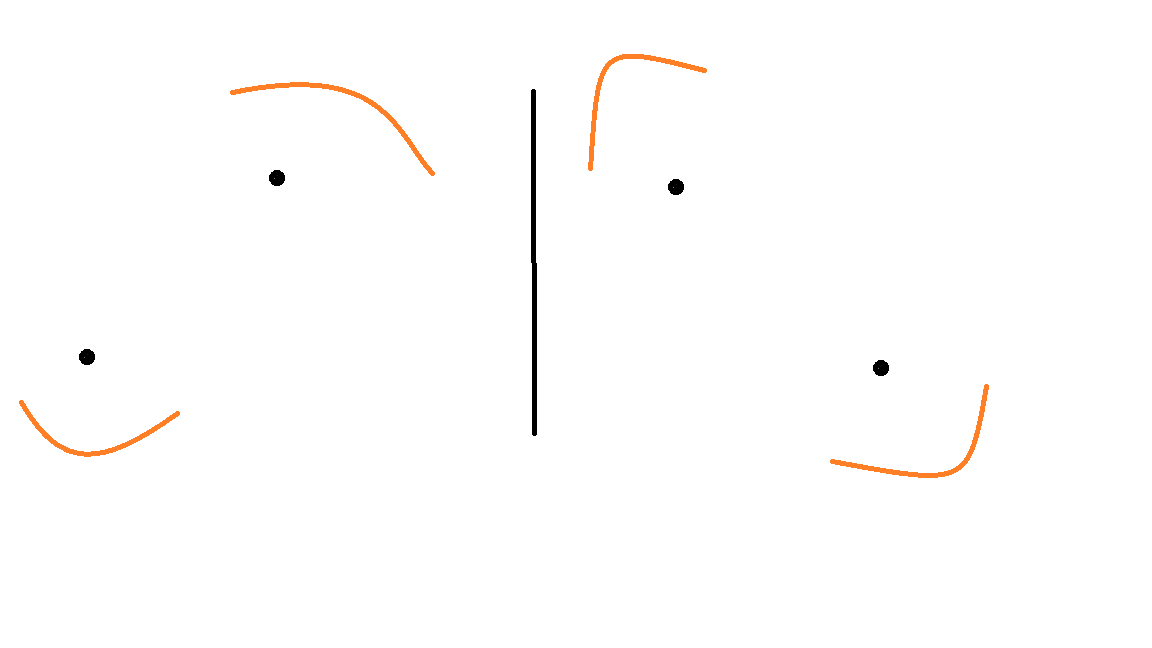
\includegraphics[width=0.4\textwidth, height=0.2\textheight]{base_case_2}}
	\caption{Base case for 2 points}
	\label{base_case_2}
\end{figure}

To consider the base case of $3$ points, we introduce an additional notion of the tangent slope given by two points on the plane. For arbitrary points $a_1, a_2$ such that $x(a_1)<x(a_2)$ slope is denoted as $\lambda$:

\begin{equation}
\lambda(a_1, a_2)=\frac{y(a_2)-y(a_1)}{x(a_2)-x(a_1)}
\end{equation}

According to this definition, the possible cases for points $a_1,a_2,a_3$ are given in table. 1 and shown in fig. 3:

\begin{table}[htbp]
	\caption{Position of 3-points base case}
	\begin{center}
		\begin{tabular}{|c|c|c|c|}
			\hline
			\textbf{$\lambda(a_1, a_2) > \lambda(a_2, a_3)$} & \textbf{$y(a_1) < y(a_2)$} & upper sub-hull & lower sub-hull \\
			\hline
			false & false & $a_1, a_3$ & $a_2$ \\
			\hline
			false & true & $a_1, a_3$ & $a_2$ \\
			\hline
			true & false & $a_2, a_3$ & $a_1$ \\
			\hline
			true & true & $a_1, a_2$ & $a_3$ \\
			\hline
		\end{tabular} 
	\end{center}
\end{table} 


\begin{figure}[htbp]
	\centerline{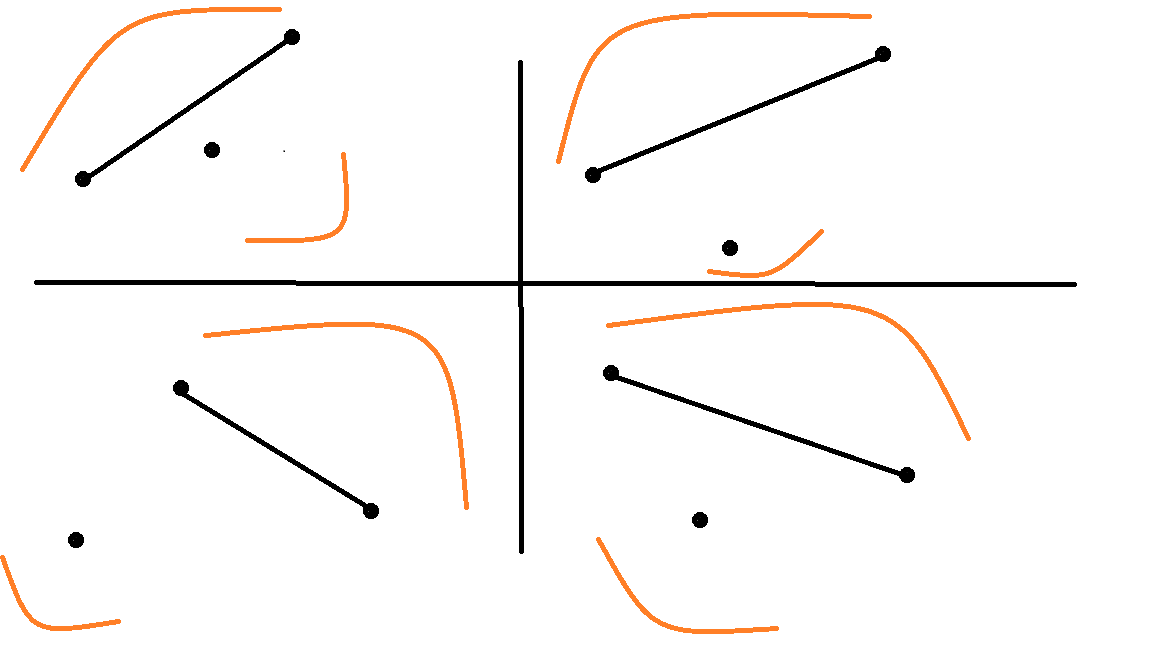
\includegraphics[width=0.4\textwidth, height=0.2\textheight]{base_case_3}}
	\caption{Base cases for a set of 3 points}
	\label{base_case_3}
\end{figure}


\subsection{The merge step}

\cite{overmars} provides an algorithm for merging two convex hulls. The essence of the algorithm is to maintain the hull with the help of two concatenated queues. The hull is divided into two parts. In this article, the separation occurs from top to bottom. Then, using the two-pointer technique and the cases described in \cite{overmars}, the proper tangent line is searched. It remains to split the two queues at the 2 found vertices that form the tangent and to merge the remaining parts. An example of performing such a procedure is shown in fig. 4.

\begin{figure}[htbp]
	\centerline{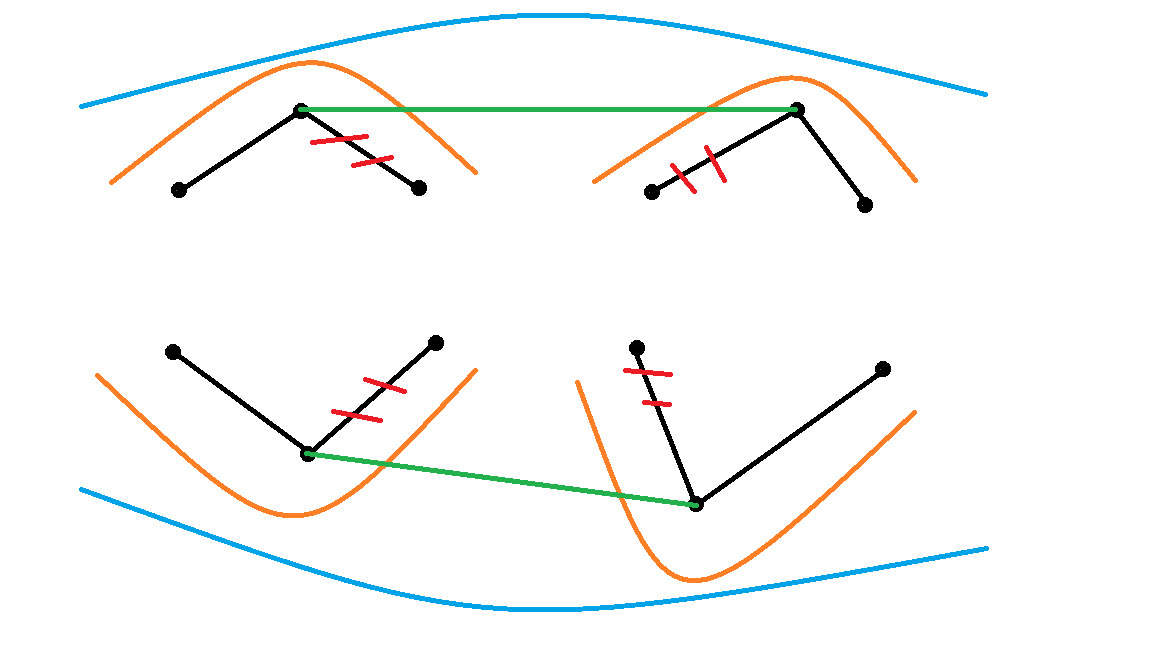
\includegraphics[width=0.4\textwidth, height=0.2\textheight]{ch_union}}
	\caption{Merging step of two hulls}
	\label{ch_union}
\end{figure}

It remains to consider the corner cases that arise when performing the merging. The first of these cases is related to the ambiguity of the position of the utmost points in the described representation of the convex hull. The leftmost point of the left hull and the rightmost point of the right hull must belong to the upper parts of the view before finding the tangent line, because otherwise such tangent may be found incorrectly. An example of such incorrect search is given in fig. 5.

\begin{figure}[htbp]
	\centerline{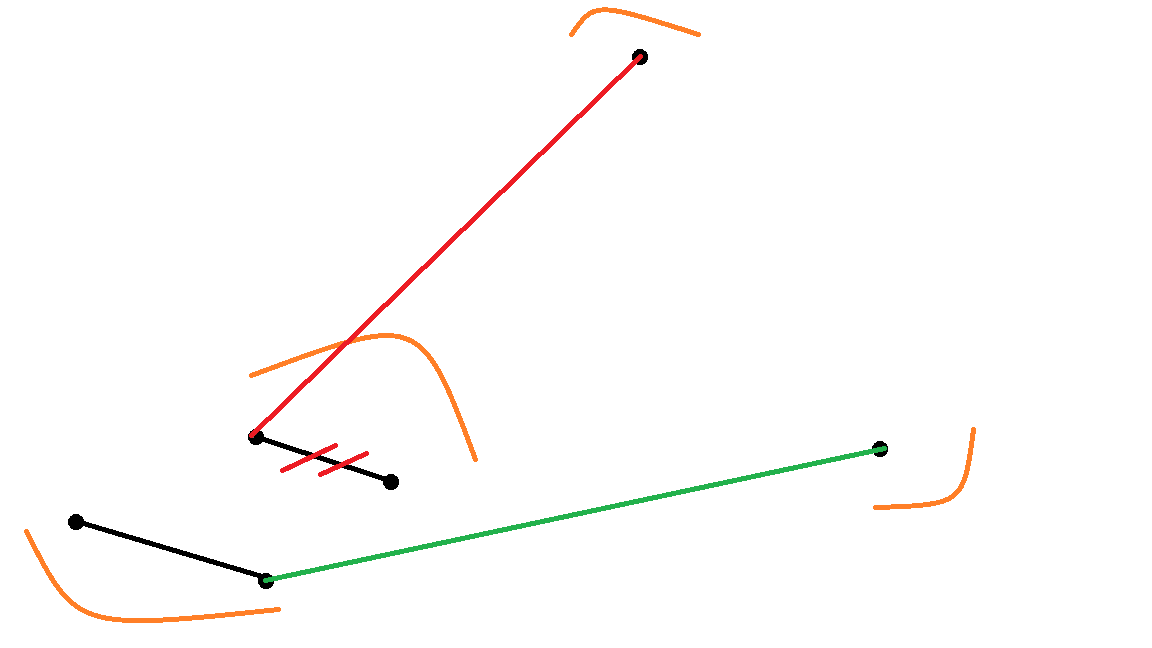
\includegraphics[width=0.4\textwidth, height=0.2\textheight]{incorect_search}}
	\caption{Example of an incorrect position of the utmost left in the left sub-hull}
	\label{incorect_search}
\end{figure}

To avoid such a situation, it is necessary to move the indicated points of their upper parts before merging the sub-hulls.

For the rightmost point of the left hull and the leftmost point of the right hull we have the following cases. Similarly to the previous argument, they must be transferred to the upper parts of the hulls. And after merging these points must be transferred to the lower parts of the hull, if they do not belong to the created upper part of the final hull. Otherwise, the formed hull may be incorrect. An example of such case is shown in fig. 6.


\begin{figure}[htbp]
	\centerline{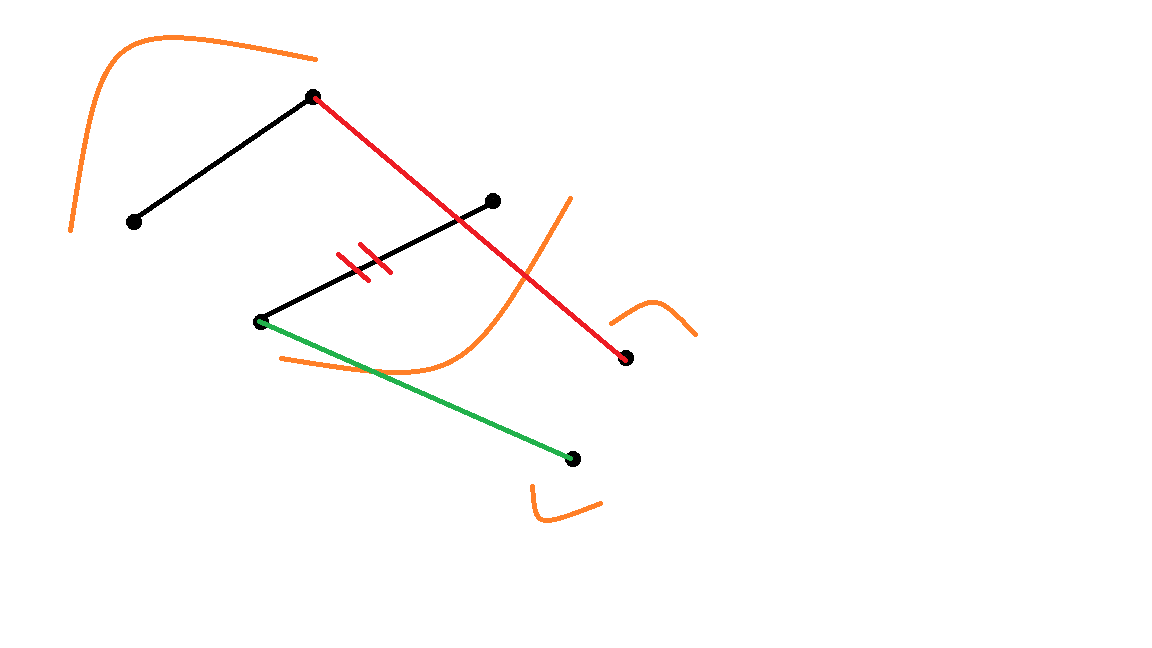
\includegraphics[width=0.4\textwidth, height=0.2\textheight]{incorect_edge_points}}
	\caption{Example of a convex hull for a wrong position of the utmost left points of the left sub-hull}
	\label{incorect_edge_points}
\end{figure}

After combining the parts of the convex hulls, another corner case might take place. The search for the tangent for the upper parts of the hulls does not take into account the position of the lower parts and vice versa. As a result, the upper and lower parts of the final hull may not form a coherent structure. An example of such a situation is shown in Fig. 7.

\begin{figure}[htbp]
	\centerline{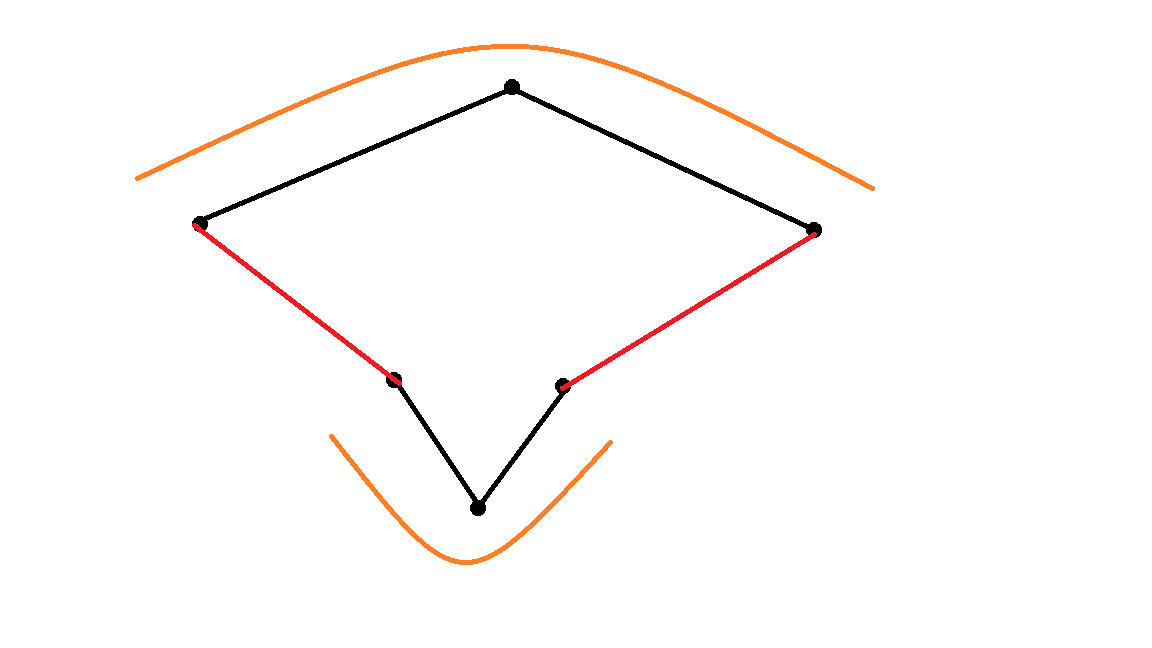
\includegraphics[width=0.4\textwidth, height=0.2\textheight]{incorect_lower_subhull}}
	\caption{An example of a non-integral hull after merging along the reference lines}
	\label{incorect_lower_subhull}
\end{figure}

To avoid such a situation, it is necessary to perform the step of cutting off the redundant parts of the formed lower sub-hull. Then searching for the left and right pivoting vertices in the concatenable queue is performed. After that, the queue is splits over the found vertices.

The cases corresponding to the left search are shown in fig. 8, and those corresponding to the right - in fig. 9. Fig. 10 shows correctly constructed convex hull.

\begin{figure}[htbp]
	\centerline{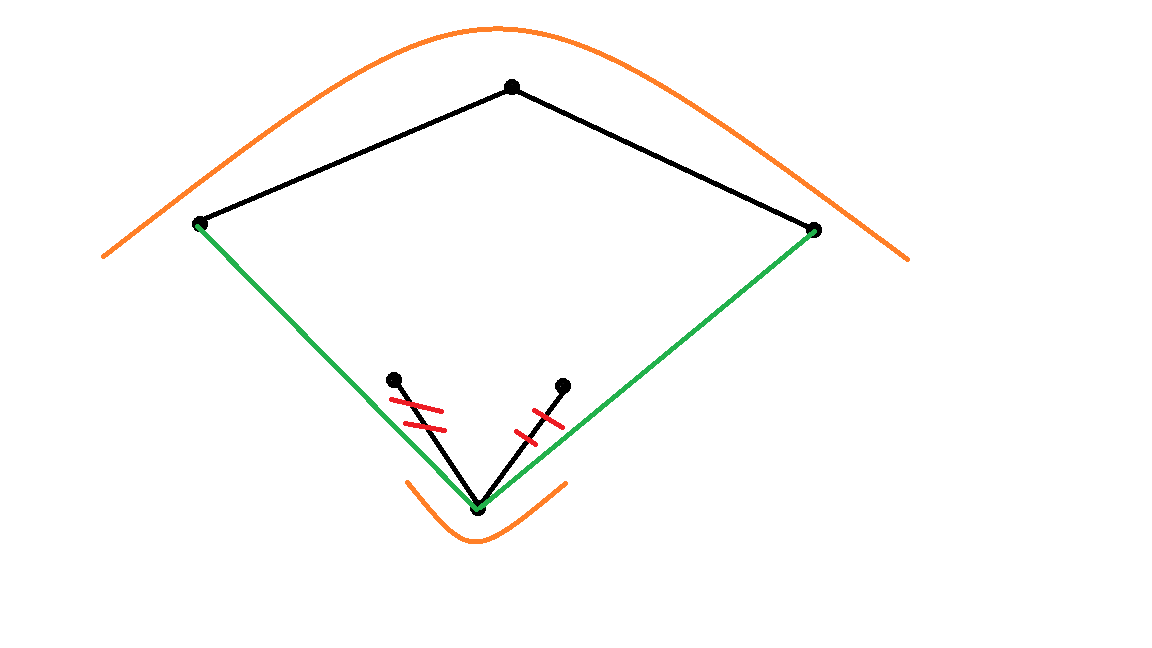
\includegraphics[width=0.4\textwidth, height=0.2\textheight]{correct_convex_hull}}
	\caption{Correctly constructed convex hull}
	\label{correct_convex_hull}
\end{figure}


\subsection{Algorithm complexity}

\begin{theorem}
	The complexity of the described convex hull construction algorithm for a static set of points is $O(n\log n)$ with sequential execution.
\end{theorem}

\begin{proof}
	We will argue the complexity of the algorithm by listing the complexities of the main stages it consists of.
	
	\begin{itemize}
		\item
		Precomputation $O(n\log n)$.
		\item
		Recursive descent and splitting the set into 2 parts $O(1)$.
		\item
		Recursive ascent and merging parts of the convex hull $O(\log n)$.
		\begin{itemize}
			\item
			Transfer of the utmost points to upper parts of convex hulls $O(\log n)$.
			\item
			Finding the tangent for the upper parts of the hulls $O(\log n)$.
			\item
			Splitting and merging the upper parts $O(\log^2 n)$.
			\item
			Moving the utmost points to the bottom of the hulls $O(\log n)$.
			\item
			Finding the tangent for the upper parts of the hulls $O(\log n)$.
			\item
			Splitting and merging the upper parts $O(\log^2 n)$.
			\item
			Merging the lower parts of the hull $O(\log n)$.
			\item
			Normalization of the obtained lower part $O(\log n)$.
		\end{itemize}
	\end{itemize}
	
	The complexity of pre-processing directly depends on the complexity of the sort algorithm . Using fast sorting algorithms \cite[page~159]{cormen}, this procedure can be performed in the optimal time of $O(n\log n)$.
	
	To estimate the complexity of the recursive procedure for constructing a convex hull, we make the following equation:
	
	\begin{equation*}
	T(n) = 2T(\frac{n}{2}) + O(\log^2 n)
	\end{equation*}
	
	According to the well-known result from the theory of algorithmic complexity we have that the solution of this equation is:
	
	\begin{equation*}
	T(n)=O(n)
	\end{equation*}
	
	Thus, taking into account the pre-processing, we get the total complexity of the algorithm $O(n\log n)$
\end{proof}

\begin{theorem}
	The complexity of the recursive convex hull construction is $O(\log^3n)$ when executed concurrently on $\frac{n}{2}$ processors.
\end{theorem}

\begin{proof}
	The recursion tree has a height of no more than $\log n$ levels. At the lowest level, the number of subtasks created is $\frac{n}{2}$. Thus, each subtask takes not more than $\frac{n}{2}$ time.
	
	
	Next, $O(\log^2 n)$ work is performed at each level. Having the height of the recursion tree, we get the total complexity of the algorithm
	
	\begin{equation*}
	T(n) = O(\log^3 n)
	\end{equation*}
\end{proof}

\section{Single algorithmic environment}

\subsection{Divide and conquer algorithm interface}

The next goal of this work is to build a single algorithmic environment. The construction of such an object requires the combination of an algorithmic database together with the necessary data structures. It will allow to incorporate all implemented algorithms together, without necessity to know their internal implementation. In fact, it is necessary to create an interface of generic algorithm based on divide and conquer strategy, which will then be used on a specific set of input data.

We start creating the generic interface by listing its components:

\begin{itemize}
	\item 
	Precomputation.
	\item 
	Splitting task into sub-tasks.
	\item 
	Solving sub-tasks.
	\item 
	Merging obtained results.
	\item 
	Checking, if a given input data is a base case for the algorithm.
	\item 
	Solving the base case.
\end{itemize}

Each of these components will represent a function of the future interface. Here there is a clear separation between the input type for the algorithm and the type of result it returns. These two types should be parameters of the algorithm model to be built. One should also pay attention to the types of functions input and output types of the interface.

A large number of computational geometry algorithms, such as computing minimal spanning tree, the Delaunay triangulation, the Voronoi diagram and the convex hull accept the list of points. However, it is not possible limit the type of input to the algorithm interface in a single algorithmic environment. The reason for this is that some algorithms can use the results of other algorithms as input data. A well known example is the construction of a Delaunay triangulation given the Voronoi diagram represented in a special data structure \cite[pp.~209]{shamos}.

Listing 6 shows the constructed algorithm model:

\begin{lstlisting}[caption={Algorithm model based on the divide and conquer principle},captionpos=b]
interface DaCAlgorithm[IT, OT]:
boolean isBaseCase(IT input)
int inputSize(IT input)
OT solveBaseCase(IT input)
OT merge(OT first, OT second)
Pair[IT, IT] divide(IT input)
IT precompute(IT input)
\end{lstlisting}

\subsection{Sequential and parallel execution}

Although this model very accurately describes the class of algorithms, it does not make it possible to solve the problem directly by having input data, which in fact enables to the algorithm from how it will be executed. In this part of the article, principles of sequential and parallel execution are considered.

When executing sequentially an algorithm, its individual subtasks computed one by one. Such algorithm is shown in Listing 7:

\begin{lstlisting}[caption={Sequential execution algorithm},captionpos=b]
OT solveRecursively(IT input,
 DaCAlgorithm[IT, OT] algorithm):
if algorithm.isBaseCase(input):
return algorithm.solveBaseCase(input)

Pair[IT, IT] p = algorithm.divide(input)
IT left = p[0]
IT right = p[1]

OT leftResult = solveRecursively(left)
OT rightResult = solveRecursively(right)

return algorithm.merge(leftResult, rightResult)
\end{lstlisting}

In parallel execution, it is necessary to take into account that the individual subtasks can be calculated independently, which significantly speeds up the execution of the algorithm.

To construct the concurrent algorithm, we use the following parallel computation abstraction $computeInParallel(function1, function2)$, which runs the functions $function1$ and $function2$ in parallel.

Listing 8 contains the main steps of this implementation.

\begin{lstlisting}[caption={Parallel execution algorithm},captionpos=b]
OT compute(IT input, 
DaCAlgorithm[IT, OT] algorithm):
if algorithm.isBaseCase(input):
return algorithm.solveBaseCase(input)

Pair[IT, IT] p = algorithm.divide(input)
IT left = p[0]
IT right = p[1]

OT leftResult,rightResult = 
computeInParallel(solveRecursively(left),
solveRecursively(right))

return algorithm.merge(leftResult, rightResult)
\end{lstlisting}

From the standpoint of the practical implementation the performance of such algorithm was improved bt introducing a limit on the size of subtasks that can be calculated in parallel.

\subsection{Performance comparison}

A number of algorithm performance measurements were performed for different input sizes and the average number of recursive tasks per thread. The results are shown in Table. 2 and 3.

\begin{table}[htbp]
	\caption{Sequential execution performance}
	\begin{center}
		\begin{tabular}{|c|c|c|c|}
			\hline
			\textbf{Number of points} & 1000000 & 10000000 & 10000000 \\
			\hline
			&52.207 (ms)&648.621 (ms)&1302.485 (ms)\\
			\hline
		\end{tabular} 
	\end{center}
\end{table} 


\begin{table}[htbp]
	\caption{Parallel execution performance}
	\begin{center}
		\begin{tabular}{|c|c|c|c|}
			\hline
			\textbf{NosptNop} & 1000000 & 10000000 & 10000000 \\
			\hline
			20 &52.434 (ms)&458.921 (ms)&969.243 (ms)\\
			
			\hline
			30 &53.615 (ms)&472.127 (ms)&845.707 (ms)\\
			
			\hline
			40 &52.797 (ms)&464.418 (ms)&907.498 (ms)\\
			
			\hline
			50 &53.189 (ms)&474.804 (ms)&905.952 (ms)\\	
			\hline
		\end{tabular} 
	\end{center}
\end{table}

\section*{Conclusion}

As a result of the work, existing methods for constructing a convex hull were analyzed and a new algorithm was proposed to solve this problem for a static set of points. A unified algorithmic environment was also created on the basis of divide and conquer algorithms, which allows to develop efficient implementation of such algorithms quickly and enables to execute them both sequentially and in parallel. The described object was implemented in Java software using standard library tools. Additionally, a tool was developed to visualize the results of the convex hull construction.

The implemented of data structures and other elements are does not use other libraries. This makes it independent and easy to use.

The main advantages of the developed algorithm are the optimization of the preprocessing stage and the effective application of such data structures as the concatenable queue, which allows to spend minimum time for the merging step of the convex hulls construction. In the preprocessing stage constant memory usage is achieved.

The performance comparison of the developed algorithm for both types of execution allows to conclude that it has high degree of parallelism. The speedup was $31\%$ percent in the best case. It is worth noting that the use of parallel execution is only necessary for very large input data.

The architecture of the created algorithmic environment makes it easy to expand its capabilities: add new as well as modify existing algorithms, implement the necessary data and extend the programmatic representation of the algorithm based on the divide and conquer scheme. This flexibility of the software product is achieved by using the modular principle in its design. In the future, it is necessary to investigate the possibility of performing parallel preprocessing. The basis for this research is given in \cite{parallel_merge_sort}.

The results of this work can be incorporated in the development of modern high-precision 3D models. The concept of a single algorithmic environment has proven to be highly relevant and effective for constructing a software for solving complex problems of computational geometry. This, along with the ease of extending the product created, makes research in this area extremely relevant.


\begin{thebibliography}{00}
	\bibitem{jarvis} Jarvis, R. A. (1973). ``On the identification of the convex hull of a finite set of points in the plane'' Information Processing Letters. 2: 18–21. DOI=10.1016/0020-0190(73)90020-3
	
	\bibitem{graham} 
	Graham, R.L. (1972). 
	``An Efficient Algorithm for Determining the Convex Hull of a Finite Planar Set'' Information Processing Letters. 1 (4): 132–133. DOI=10.1016/0020-0190(72)90045-2
	
	\bibitem{quickhull} 
	Barber, C. Bradford; Dobkin, David P.; Huhdanpaa, Hannu (1 December 1996).
	``The quickhull algorithm for convex hulls''
	ACM Transactions on Mathematical Software. 22 (4): 469–483. DOI:10.1145/235815.235821 
	
	\bibitem{preparata} 
	F. P. Preparata and S. J. Hong. 1977. 
	``Convex hulls of finite sets of points in two and three dimensions''
	Commun. ACM 20, 2 (February 1977), 87-93. DOI=10.1145/359423.359430
	
	\bibitem{overmars}
	Overmars, Mark H. and Jan van Leeuwen.  
	``Maintenance of Configurations in the Plane''
	J. Comput. Syst. Sci. 23 (1981): 166-204.
	
	\bibitem{aho}
	Alfred V. Aho 
	``The Design and Analysis of Computer Algorithms'' (1st ed.). / John E. Hopcroft., John E. Ulman. -
	Addison-Wesley Longman Publishing Co., Inc., Boston, MA, USA 1974. ISBN 0201000296
	
	\bibitem{cormen}
	``Introduction to Algorithms'' / (3rd ed.).
	[Cormen, Thomas H., Leiserson, Charles E., Rivest, Ronald L., Stein, Clifford] (2009) - MIT Press and McGraw-Hill.\\ ISBN 0-262-03384-4.
	
	\bibitem{parallel_merge_sort} Richard Cole. 1988.  
	``Parallel merge sort'' SIAM J. Comput. 17, 4 (August 1988), 770-785. DOI=10.1137/0217049
	
	
	\bibitem{shamos}
	Franco P. Preparata and  Michael I. Shamos. ``Computational Geometry: an Introduction'' - Springer-Verlag, Berlin, Heidelberg 1985.
	ISBN 0-387-96131-3
	
	\bibitem{tarjan}
	Cheriton, David R. and Robert E. Tarjan.
	``Finding Minimum Spanning Trees''
	SIAM J. Comput. 5 (1976): 724-742.	
\end{thebibliography}
\end{document}
